\documentclass{article}
\usepackage[includeheadfoot,margin=1.0in]{geometry}
\usepackage{amsfonts}
\usepackage{amsmath}
\usepackage{amssymb}
\usepackage{fancyhdr}
\usepackage{hyperref}
\usepackage{graphicx}

\title{Software Design Document}
\author{Team USA \\ Software Engineering \\ Sam Houston State University}

\pagestyle{fancy}
\fancyhead[LE,RO]{OpenSSL}
\fancyhead[RE,LO]{\leftmark}
\fancyfoot[RE,LO]{}
\renewcommand{\headrulewidth}{2pt}
\renewcommand{\thefootnote}{[\arabic{footnote}]}
\begin{document}
% Generate Title
\maketitle
\newpage

% Generate Table of Contents
\tableofcontents
\newpage

% Begin Design Document Content
% Begin Section 1 - Top Down Iterative Refinement
%
\section{Design \#1: Top Down Iterative Refinement}
	\subsection{General Considerations}
	\subsection{Metrics}
	\subsection{Analysis}
	\subsection{Conclusion}
%
% End Section 1, Begin Section 2 - Dynamic Data Flow Analysis
%
\section{Design \#2: Dynamic Data Flow Analysis}
	\subsection{General Considerations}
		Dynamic data flow analysis is a design methodology used to demonstrate the flow of data through a software system. A good software design, when analyzed with the dynamic data flow method will show a well defined input, or afferent, branch where data is collected and acted upon by related input processing functions (such as opening a file or reading the file contents to an array for use by another module). Data processed by the afferent branch should then be passed to a well defined central transform branch where the core operations of the software are performed on the data, and output data is generated and returned. Finally, this output data is sent a well defined output, or efferent, branch, where it is processed into its final output format, such as a report. 
	
		Two data flow diagrams are used when plotting the path of data from input to output in a software system. The first is a flow diagram, which shows data coming into the system, how it moves through the system's various modules, and eventually is output in a useful way. The second diagram is a hierarchical diagram that shows the modules that make up the system, and how they are related. This diagram shows the flow of data, but also implies the control structure of each module as it relates to the others and to the system as a whole. Data couples and control couples are indicated here as well. Further, because this type of analysis focuses on the flow of data, with an implied control structure and without any concern for the contents of the actual function bubbles present in the diagram, it is not able to determine or show the cohesiveness of any particular module. This is detrimental because it potentially allows modules that are merely coincidentally cohesive to exist until the implementation phase, when the problems associated with that form of cohesion will likely begin to appear. 
	\subsection{Analysis Metrics}
		\subsubsection{Coupling}
			Dynamic data flow analysis focuses on two types of coupling: data and control.\footnote{See Appendix A, Section 5.2, Subsection 5.2.2 for the appropriate diagram, demonstrating coupling.} 
			\paragraph{Data Coupling}
				Data coupling occurs when one module depends on the output of another, and the data they exchange is composed of discreet, elementary units, providing exactly what each module needs and nothing more or less. This is the lowest form of coupling with the least dependency between coupled modules. 
			\paragraph{Control Coupling}
				Control coupling occurs when one module's output is used to influence or determine the execution logic of a subsequent module - for example, a boolean value or control flag is passed from one module into another that performs a different action depending on the value it receives. This type of coupling is detrimental to the software system because it implies that each of the coupled modules must know something about what is contained in the other, meaning one or both may not be a true black box, which indicates that one or both may not be separately implementable or maintainable. 
		\subsubsection{Miller's Law}
			Miller's law tells us that, on average, the largest number of tasks that can be simultaneously held in memory is $7\pm2$. Thus, we should work for a design wherein each module complies with this law and its value. Using dynamic data flow analysis, we can see how the data flows into and out of each module, and with the hierarchical model, how control is implied to flow between modules as well. A good design will show, on average, each module having 4 to 5 tasks, and not more than $7\pm2$.\footnote{See softEng1.docx, page 36, by David Burris for more information on Miller's Law.}  
		\subsubsection{Graciunas's Law}
			Graciunas's law concerns itself with the number of control relations between modules, and predicts how this impacts the complexity of the software system. For a given set of modules, $R$, we have that $R = M(2^{M-1} + M - 1)$, where $M$ is the number of subordinate modules. Because dynamic data flow analysis shows the flow of data and the implied flow of control throughout the system, we can use this law and its equation to minimize the number of inter-module relations to the ideal minimum, represented by the equation 
			$$I = \frac{N(N - 1)}{2}$$
			where $I$ is the number of interactions between modules and $N$ is the number of modules in the system. \footnote{See softeng1.docx, page 40, by David Burris for more information on Graciunas's Law.}
		\subsubsection{Factoring}
			Factoring of a system occurs when the system is divided into an upper level of control modules, controlling a lower level of operations modules. Systems that are highly factored have few upper level modules and more lower level modules, and take on a hierarchical form. Further, highly factored systems should ideally be organized such that a set of input modules collect and organize input to pass to a central transform branch, which processes the data taken from the input, or afferent, modules, and sends it to a collection of output, or efferent, modules for final formatting and output back to the user.\footnote{See softeng2.docx, page 11, by David Burris for more information on factoring.} 
		\subsubsection{Scope of Control}
			Scope of control in an organized, factored system is a measurement of the control of superordinate modules against subordinate modules. Ideally, the scope of control should be such that decisions made by a superordinate module \emph{only} effect its direct subordinates, and no other modules in the system. This insures that during maintenance and modification, debugging, and testing, problems or errors caused by one module will not have a ripple effect on other, unrelated modules in the system. This simplifies debugging and maintenance and modification, thus reducing complexity, cost, and time devoted to fixing errors.\footnote{See softeng2.docx, page 13, by David Burris for more information on Scope of Control.}  
		\subsubsection{Black Boxes}
			A module is defined as a true black box whenever the module can be fully utilized with no regard for its construction, and when it performs the same action or function for every invocation, without regard to its inputs or outputs. Dynamic data flow can show the existence of black boxes in a design by showing how the inputs to a module relate to its outputs.\footnote{See softeng1.docx, page 34, by David Burris for more information on black boxes.} 
		\subsubsection{Fan-In/Out}
			Fan-in and fan-out occur when a module is a target for multiple, higher level modules, or when a module outputs to multiple, lower level modules. Fan-in is desirable because for multiple modules needing the same function, that function can be coded, debugged, and maintained once, no matter how many modules it services. However, to insure reduced complexity and cost, the module that is the target of fan-in should be a terminal module, and should be a true black box - it should perform the exact same function for every module it services. Fan-out is less desirable, because it implies a linkage between a servicing module and the serviced modules. A change in the servicing function may require changes in the modules being serviced. Further, modules with are both targets of fan-in \emph{and} fan-out are the least desirable, as there is an implied linkage between the servicing module and the serviced modules, and because the target module becomes subject to Graciunas's Law, causing complexity to rapidly increase.\footnote{See softeng2.docx, page 14, by David Burris for more information on fan-in/out} 
	\subsection{Analysis}
		The software system in question is that of a point-and-click, two dimensional game. We will draw conclusions from our analysis using both the data flow diagram and the hierarchical diagram from the previous dynamic data flow analysis of the software system. 
		\subsubsection{Coupling}
			The design exhibits high levels of data coupling between modules, and a low level of control coupling between modules. Data coupling, while potentially undesirable, is the least detrimental form of coupling, and is likely present in every software design to some degree. In general, our design is data coupled at interfaces between higher level modules and lower level modules, and the data is being passed down the hierarchy for efferent modules and up the hierarchy for afferent modules, as expected. Control coupling occurs in the design at interfaces between controller-type modules and the modules they control. Because the system is a game, it relies on certain modules to control the overall execution of the other, subordinate data processing modules. These control modules then are necessarily coupled to their subordinate processing modules. While this is undesirable from a design standpoint, it is unavoidable. 
		\subsubsection{Miller's Law}
			The design does not exhibit any modules that exceed $7\pm2$ interactions. Of concern is the \texttt{Engine} module,\footnote{See Appendix A, Section 5.2, Subsection 5.2.2 for the appropriate diagram.} which has 8 links to other modules in the system. The links are asynchronous, however, as the \texttt{Play Video Request} and \texttt{Play Audio Request} controls are not necessarily sent to the video and audio manager functions at the same time as the file paths. Thus, though the engine has 8 links to other modules, it may have between 4 and 8 actually active in a single given frame. Still, it is important to keep in mind that any further requirements on this module will therefore likely result in rapid increases in implementation, debugging, and maintenance \& modification difficulties. 
			
			Regarding the system as a whole, we know that it is desirable to maintain an average of 3 to 4 interactions between modules throughout the system as a whole, and we can perform basic math to determine where our system stands, based on the data flow diagrams we have obtained through our analysis. Thus, we can derive a table showing each module and the number of interactions it has with other modules:
			\begin{center}
				\begin{tabular}{| l || c |}
					\hline
					Get Mouse State 					& 3 \\ \hline
					Create Save File					& 3 \\ \hline
					Parse Save File 					& 3 \\ \hline
					Load Level							& 3 \\ \hline
					Engine								& 8 \\ \hline
					Update Player						& 6 \\ \hline
					Compare Player \& Actor Positions	& 2 \\ \hline
					Video Manager						& 3 \\ \hline
					Render Video						& 2 \\ \hline
					Audio Manager						& 3 \\ \hline
					Play Audio							& 2 \\ \hline
					\textbf{Total:}						& 38 \\
					\hline
				\end{tabular}
			\end{center}
			So we can calulate $A$, the average number of interactions between modules with regard to Miller's Law by dividing 38 by the number of modules $N$, where $N = 11$: 
			$$A = 45 \div N = 38 \div 11 = 3.4545$$
			Therefore, while two of the design's modules approach the limits of Miller's Law, the overall average number of interactions between modules with regard to Miller's law is within the expected range of values, at $3.4545$. 
		\subsubsection{Graciunas's Law}
			Because the design makes use of a highly factored, modular design, the majority of data is passed from one module to another, using a one-way connection where each module only communicates with its direct superior, controlling module. This insures that each pair of modules only has one path of communication between them, and thus only 1 relationship. The \texttt{Engine} module,\footnote{See Appendix A, Section 5.2, Subsection 5.2.2 for the appropriate diagram.} however, interacts with 6 modules, with two relationships between two of its subordinate modules. Thus, its number of interactions are defined by the equation $$I = \frac{N(N - 1)}{2}$$
			where $I$ is the number of interactions between modules and $N$ is the number of modules in the system:
			$$I = \frac{6(5)}{2} = 15$$
			And so \texttt{Engine} has 15 possible interactions in the system, and the system as a whole has 
			$$I = \frac{11(10)}{2} = 55$$
			Limiting data and control this way substantially reduces complexity. Not implementing this type of design results in the number of relations being defined by $R = M(2^{M-1} + M - 1)$, where $M$ is the number of subordinate modules. If we calculate that value, we have that
			$$R = 11(2^{11-1} + 11 - 1)$$
			$$R = 11(1024 + 11 - 1)$$
			$$R = 11(1034) = 11374$$
			And so we can clearly see that by limiting the number of data and control relations between modules to the absolute minimum, we have reduced the number of relations by an approximate factor $206$. 
		\subsubsection{Factoring}
			Our design is highly factored, in that we have a central module, \texttt{Engine} that delegates to another, lower level of modules, and those modules delegate to yet another level of modules. Further, we can organize the modules into afferent modules and efferent modules, all sending data to or receiving data from a central transform branch, headed by \texttt{Engine}. By having a highly factored, branched design, we can insure that each module complies with Miller's law, Graciunas's law, and that the scope of control (discussed in the next section) and scope of effect are all within the ideal parameters. Additionally, by not sending control flags back and forth between superordinate modules and subordinate modules, we have reduced control coupling to acceptable levels.\footnote{See Appendix A, Section 5.2, Subsection 5.2.2 for the appropriate diagram.}  
		\subsubsection{Scope of Control}
			If we examine the factored design diagram,\footnote{See Appendix A, Section 5.2, Subsection 5.2.2 for the appropriate diagram.} we can see how the data is being moved between modules. Each module in the design is only able to request information from the module(s) directly subordinate to it, with regard to the afferent branch. The central transform branch, consisting of the \texttt{engine} module and its two subordinate modules, only allows control decisions to be made by \texttt{Engine}, with regard to its subordinate modules. However, one issue with this design is that one of \texttt{Engine}'s subordinate modules passes back an actor event, and the type of event \texttt{Engine} receives directly determines how it proceeds in its execution with regard to that event. Thus, control in this case is moving from a subordinate module to a superordinate module, which is typically considered detrimental to the system. However, as this is the only place in the design where this occurs, and because the design is that of a game, this behavior is expected, and has been taken into account. 
		\subsubsection{Black Boxes}
			If we examine the data flow diagram\footnote{See Appendix A, Section 5.2, Subsection 5.2.1, for the appropriate diagram.}, we can see that our analysis shows extensive use of black boxes. Each module sends, receives, and processes data completely independently of other modules. Therefore, any change made in one module will not affect the data processing of any other modules, which reduces complexity. This insures that a minimum of time will be spent debugging errors and maintaining the software throughout its life. One exception here is, as discussed in the subsection covering scope of control, is \texttt{Engine}. Because it is control coupled with a subordinate module, a change in \texttt{Engine} or a change in the types of actor events it receives from its subordinate modules is subject to additional errors in whichever module was not modified. Although this behavior is expected and accounted for, it must be paid special attention during debugging and modification, to insure that the system continues to function properly. While this behavior is considered negative, it is necessary for the full functionality of the game itself, and cannot be avoided.  
		\subsubsection{Fan In/Out}
			Fan in and fan out are two features of software design that can be indicative of a design's quality. Our design makes extensive use of both. Looking at the factored diagram, we can see that the engine module is a target of fan out, indicating a factored design that delegates processing to lower level modules and control to superordinate modules. This is an ideal state for our system to be in. If we examine other modules, terminating modules, or those at the lowest levels of the system, are consistently targets for fan in, which is, again, an ideal state. For the system in question, we have an average fan out value of 6. Ideally, this value would be between 3 and 4, but it still complies with Miller's Law, which recommends not exceeding a value of $7\pm2$. 
	\subsection{Conclusion}
		While dynamic data flow analysis is a very beneficial design methodology, which clearly shows the flow of data through a system, data coupling, control coupling, and allows a designer to develop a highly factored system, it cannot measure or demonstrate the amount, level, or type of cohesion within each module. Thus, for our application of game development, it provides useful metrics, but is not ideally suited for what our design seeks to achieve. It does indicate, however, that we have developed a quality design, with high factoring, black boxes, low control coupling, moderate
data coupling, and highly differentiated and well defined afferent, efferent, and central control branches. 
%
% End Section 2, begin Section 3 - Static Data Flow Analysis
%
\section{Design \#3: Static Data Flow Analysis}
	\subsection{General Considerations}
	\subsection{Metrics}
	\subsection{Analysis}
	\subsection{Conclusion}
%
% End Section 3, begin Section 4 - Object Oriented Design
%
\section{Design \#4: Object Oriented Design (UML)}
	\subsection{General Considerations}
	\subsection{Metrics}
	\subsection{Analysis}
	\subsection{Conclusion}
%
% End Section 4, begin appendix A - Associated Diagrams & Figures
%
\section{Appendix A: Diagrams \& Figures}
	This appendix contains all of the relevant diagrams for each design methodology discussed in the SDD previously.
	\subsection{Top Down Iterative Refinement}
	\subsection{Dynamic Data Flow Analysis}
		\subsubsection{Flow Diagram}
			\begin{center}
				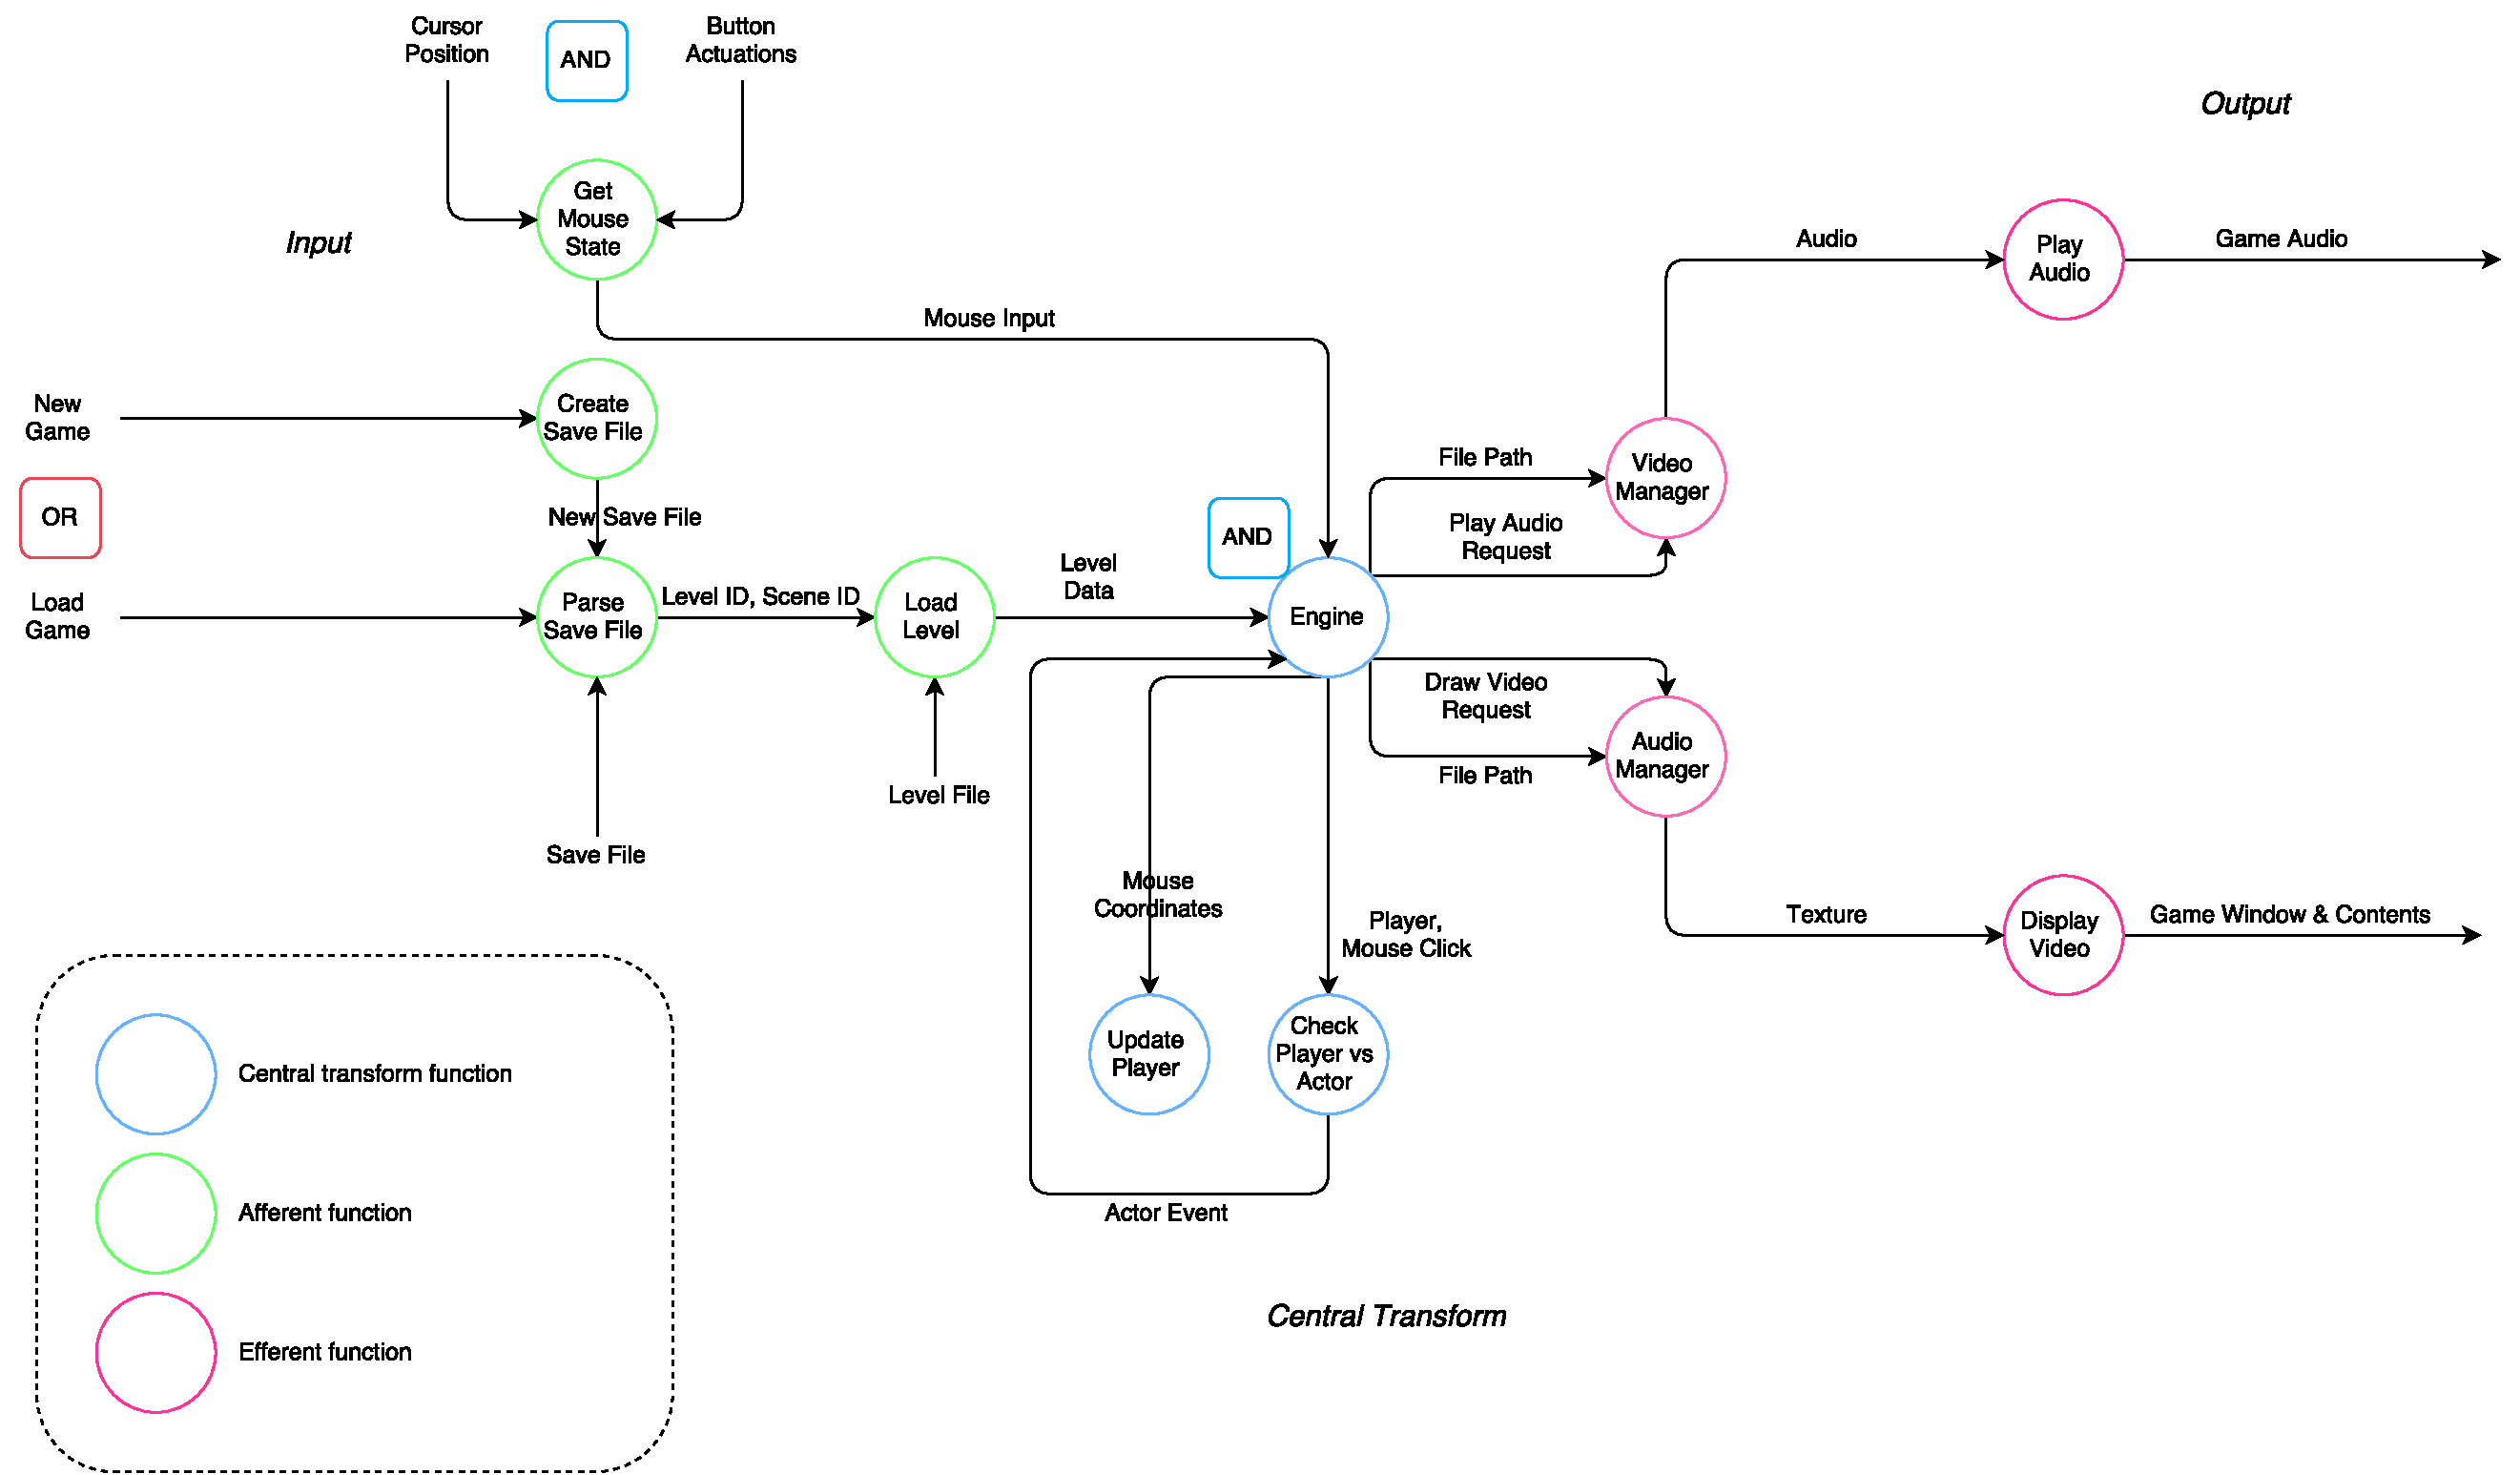
\includegraphics[scale=0.35]{ddfFlow}
			\end{center}
		\subsubsection{Factored Diagram}
			\begin{center}
				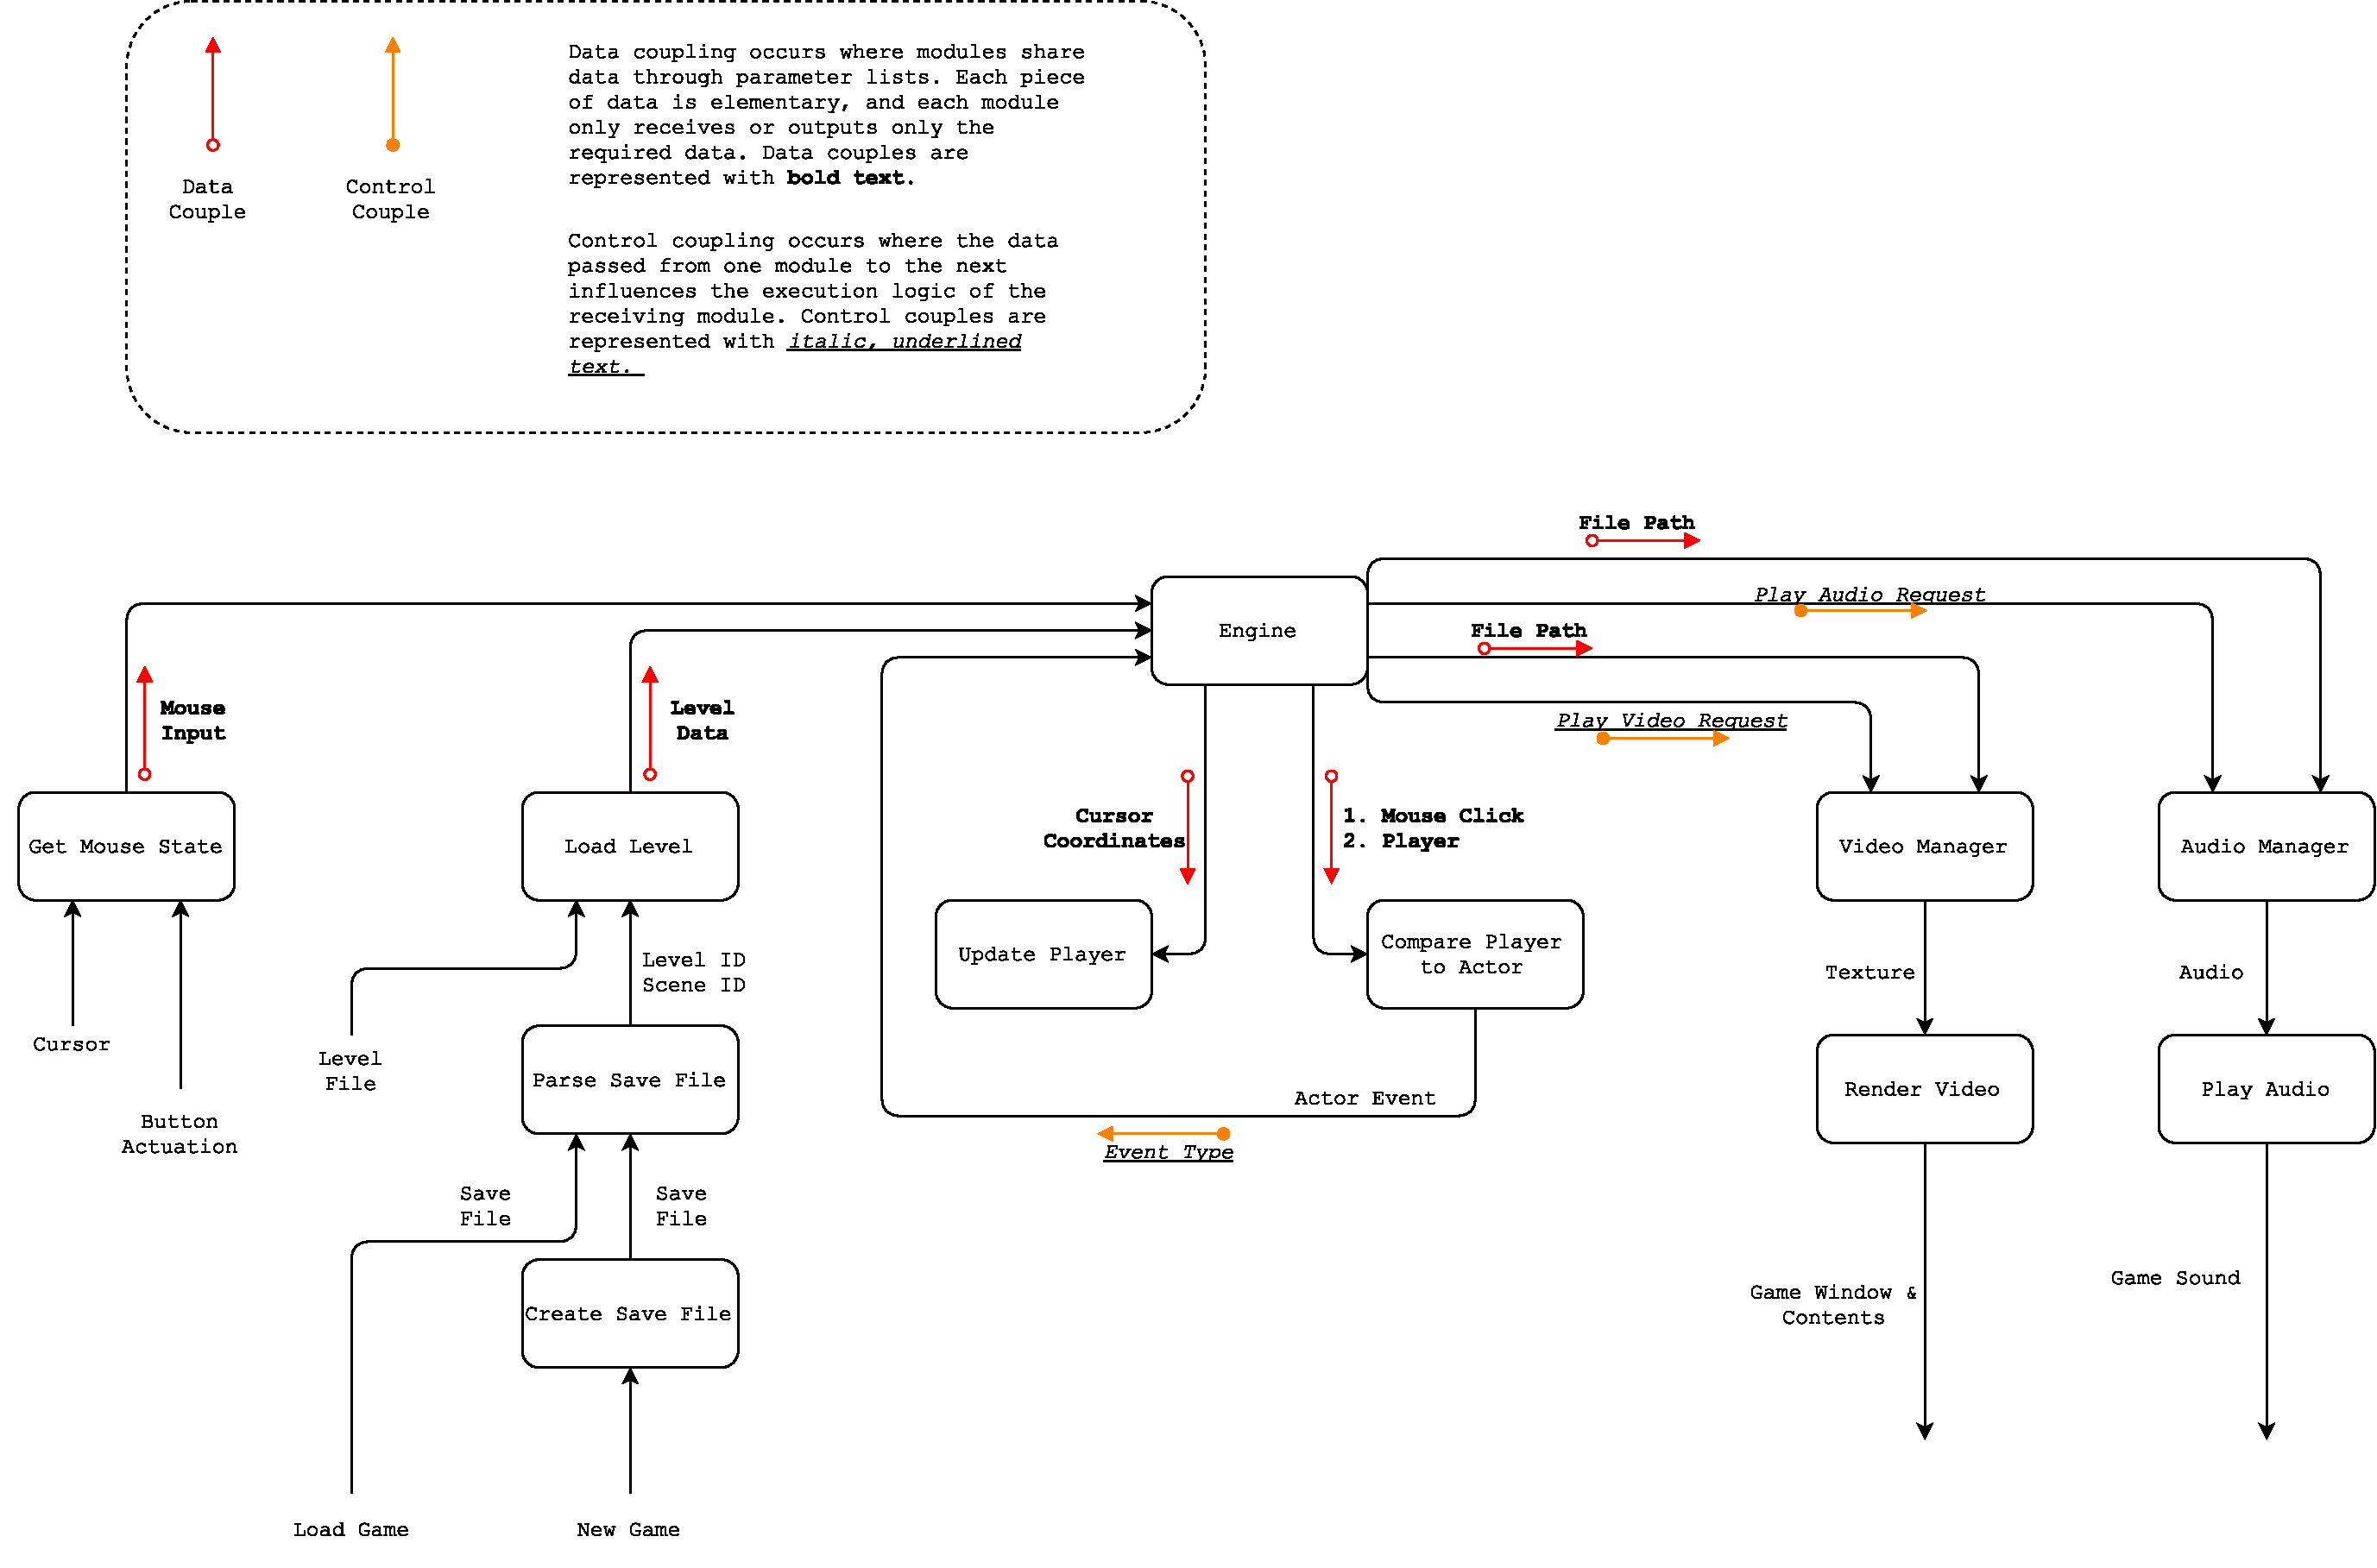
\includegraphics[scale=0.35]{ddfFactored}
			\end{center}
	\subsection{Static Design Analysis}
	\subsection{Unified Modeling Language}
		\subsubsection{UML Diagram}
			\begin{center}
				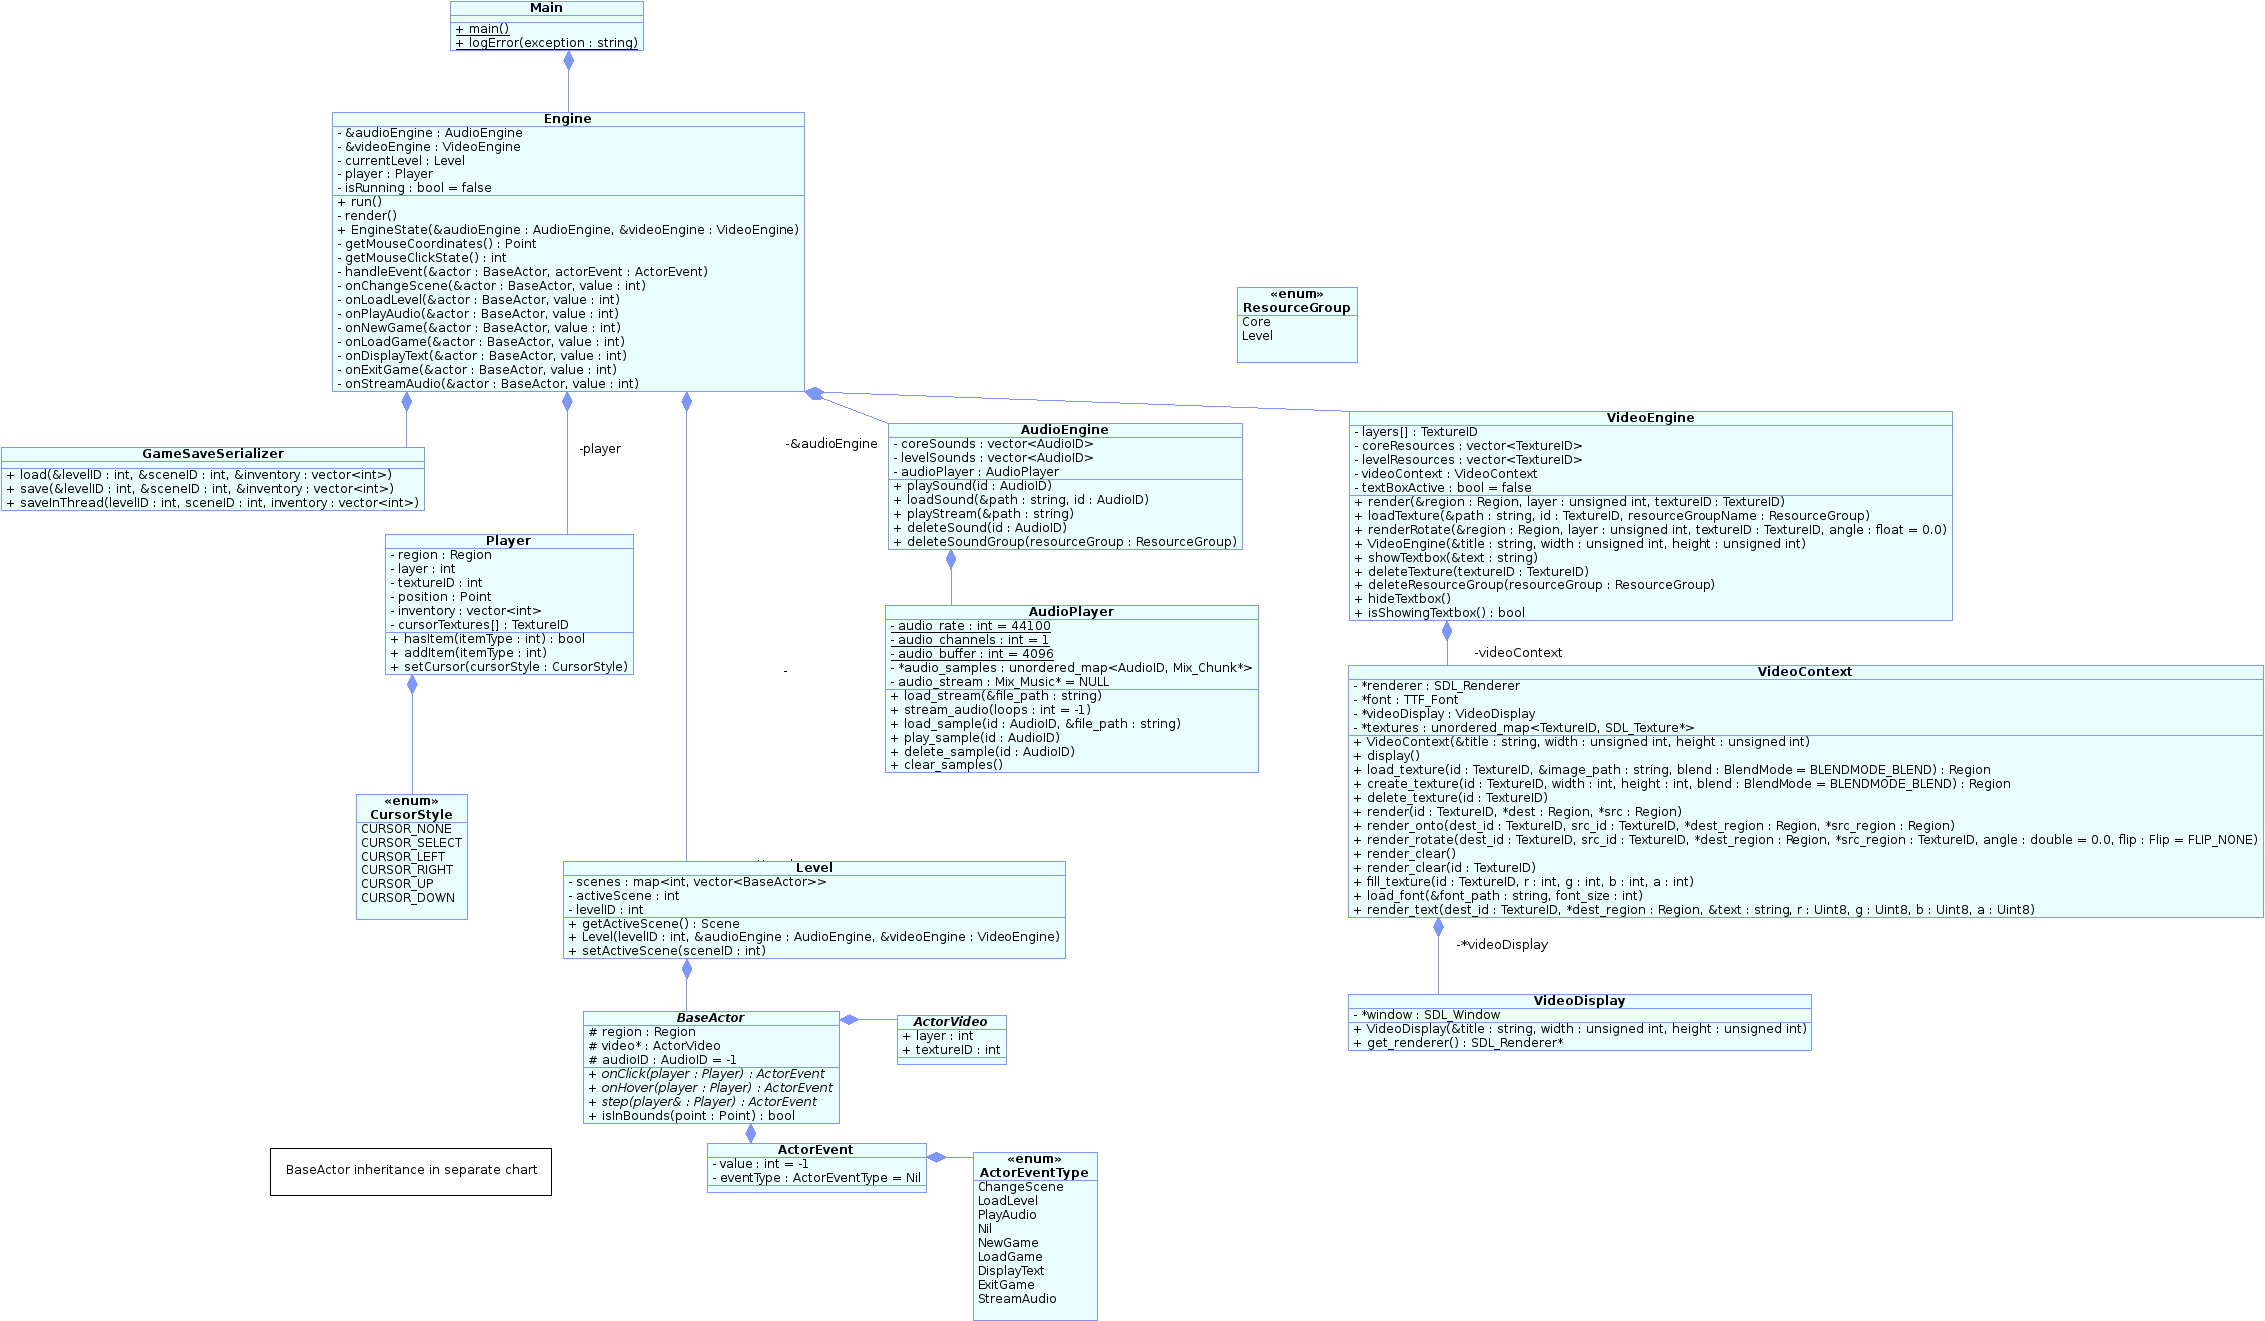
\includegraphics[scale=0.30]{MainClasses}
			\end{center}
		\subsubsection{Actor Inheritance Sub-diagram}
			\begin{center}
				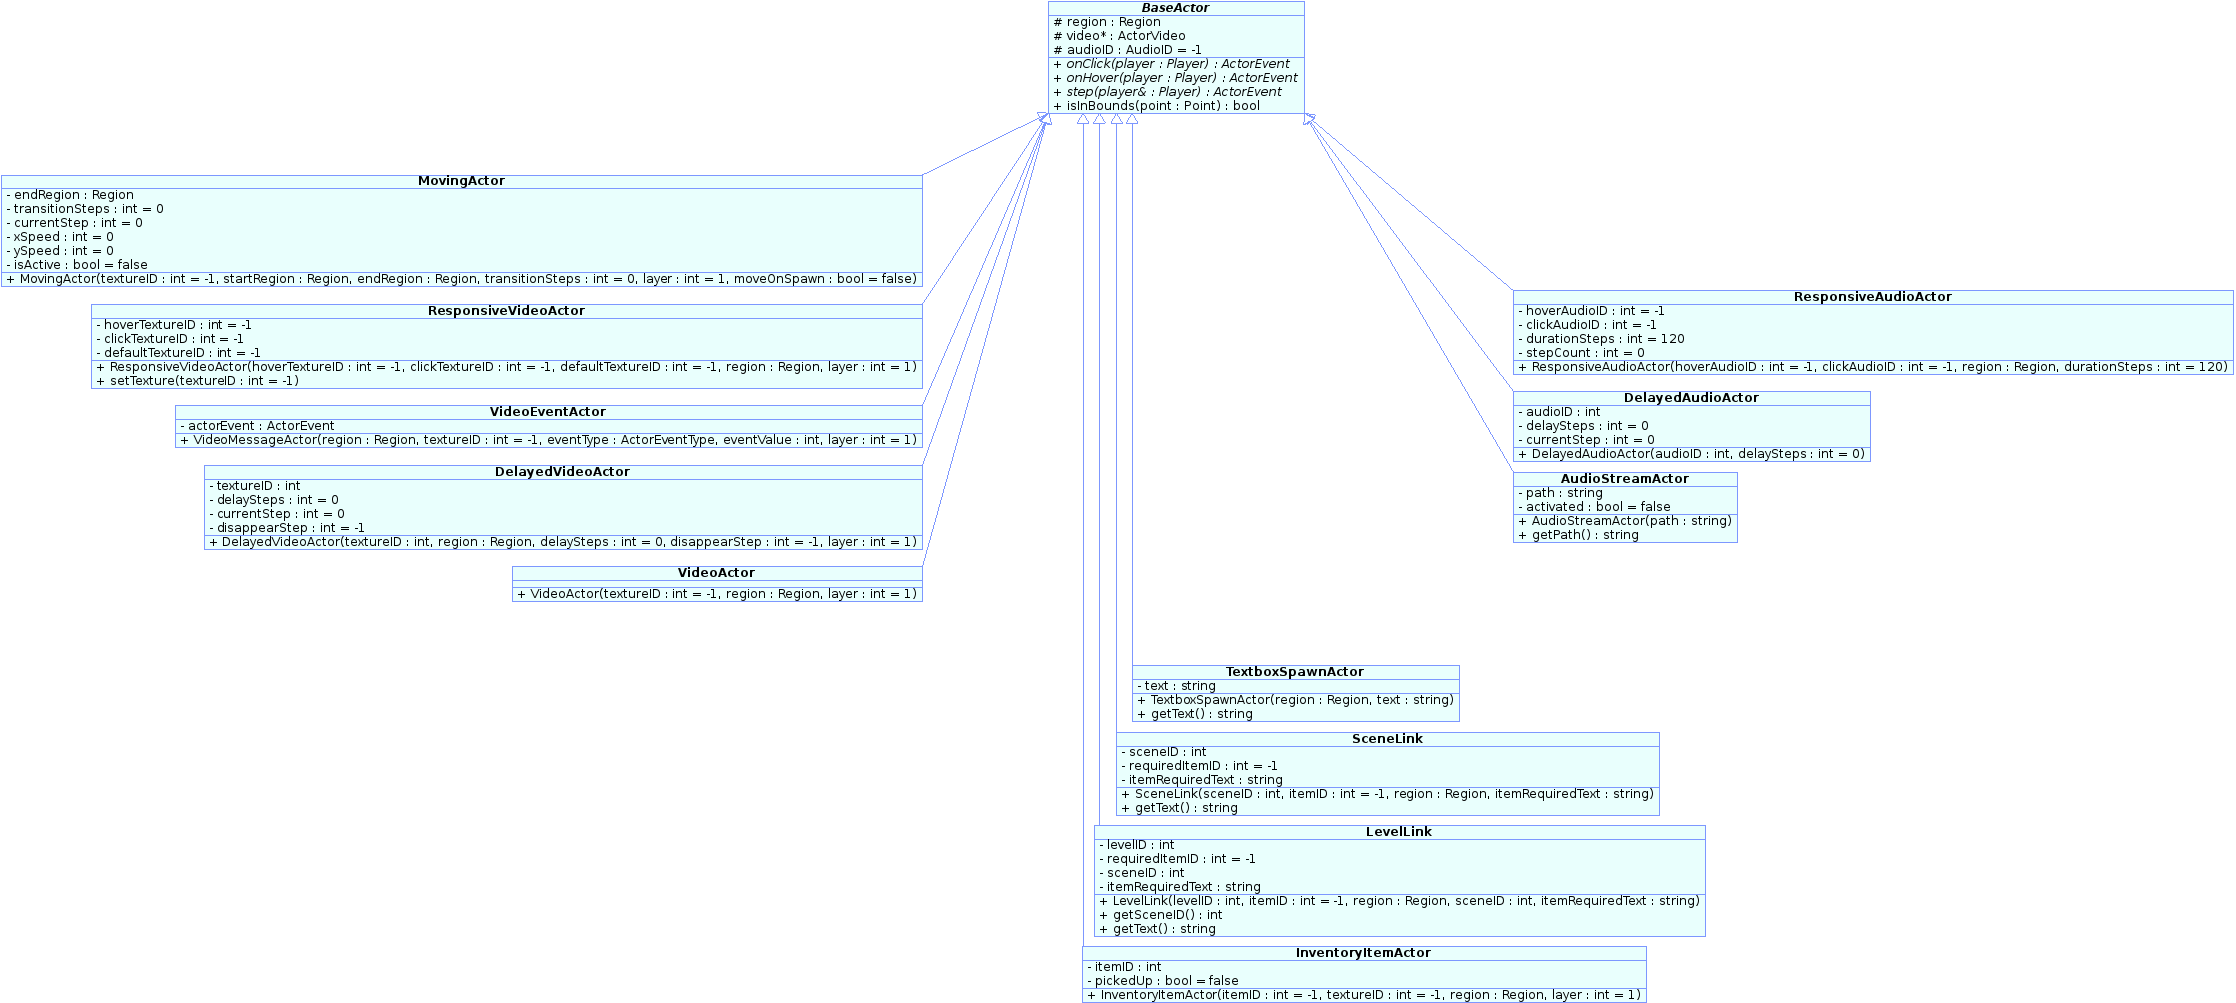
\includegraphics[scale=0.35]{Actors}
			\end{center}
		
\end{document}